% This is a self-contained tex taken from USENIX style latex template. 

\documentclass[letter,twocolumn,10pt]{article}
\usepackage[margin=1in]{geometry}
\usepackage{enumitem}
\usepackage{url}
\usepackage{makecell}
\usepackage{csquotes}
\usepackage{booktabs}
\usepackage{tabularx}
\usepackage{tikz}
\usepackage{amsmath}
\usepackage{graphicx}
\usepackage{subfig}
\usepackage{caption}
%\usepackage{subcaption}
\usepackage[numbers,sort&compress]{natbib}
\usepackage[super]{nth}
\usepackage{breakurl}
\usepackage[breaklinks]{hyperref}
\def\UrlBreaks{\do\/\do-}

\setlength{\textheight}{9.0in}
\setlength{\columnsep}{0.33in}
\setlength{\textwidth}{7.00in}
\setlength{\topmargin}{0.0in}
\setlength{\headheight}{0.0in}
\setlength{\headsep}{0.0in}
\addtolength{\oddsidemargin}{-0.25in}
\addtolength{\evensidemargin}{-0.25in}

\def\@maketitle{\newpage
 \vbox to 2.5in{
 \vspace*{\fill}
 \vskip 2em
 \begin{center}%
  {\Large\bf \@title \par}%
  \vskip 0.375in minus 0.300in
  {\large\it
   \lineskip .5em
   \begin{tabular}[t]{c}\@author
   \end{tabular}\par}%
 \end{center}%
 \par
 \vspace*{\fill}
 }
}

\begin{filecontents}{\jobname.bib}
@Book{arpaciDusseau18:osbook,
  author =       {Arpaci-Dusseau, Remzi H. and Arpaci-Dusseau Andrea C.},
  title =        {Operating Systems: Three Easy Pieces},
  publisher =    {Arpaci-Dusseau Books, LLC},
  year =         2015,
  edition =      {1.00},
  note =         {\url{http://pages.cs.wisc.edu/~remzi/OSTEP/}}
}
@InProceedings{waldspurger02,
  author =       {Waldspurger, Carl A.},
  title =        {Memory resource management in {VMware ESX} server},
  booktitle =    {USENIX Symposium on Operating System Design and
                  Implementation (OSDI)},
  year =         2002,
  pages =        {181--194},
  note =         {\url{https://www.usenix.org/legacy/event/osdi02/tech/waldspurger/waldspurger.pdf}}
}
@inproceedings{CooperSTRS10socc,
  author    = {Brian F. Cooper and
               Adam Silberstein and
               Erwin Tam and
               Raghu Ramakrishnan and
               Russell Sears},
  title     = {Benchmarking cloud serving systems with {YCSB}},
  booktitle = {Proceedings of the 1st {ACM} Symposium on Cloud Computing, SoCC 2010,
               Indianapolis, Indiana, USA, June 10-11, 2010},
  pages     = {143--154},
  year      = {2010},
  doi       = {10.1145/1807128.1807152}
}
@misc{leveldb,
    author={Google},
    title={LevelDB},
    howpublished={\url{https://github.com/google/leveldb}}
}
@misc{rocksdb,
    author={Facebook},
    title={RocksDB},
    howpublished={\url{https://github.com/facebook/rocksdb}}
}

\end{filecontents}

\begin{document}

\date{}

%-------------------------------------------------------------------------------
%TODO You should come up with a compelling title. 
\title{\Large \textbf{Report of Project 1}}
%TODO Your name. 
\author{Kai Li}
%-------------------------------------------------------------------------------
\maketitle

%-------------------------------------------------------------------------------
\section*{Abstract}
%-------------------------------------------------------------------------------
Nowadays, LevelDB has become a very popular key-store database prototype. In this project, we demonstarte on how to investigate LevelDB by running some benchmarks to show the performance under different configurations. We tune three configurable parameters and report the results, by comparing the results, we further explain how and why each option influences the system's performance.
%-------------------------------------------------------------------------------
\section{Introduction}
%-------------------------------------------------------------------------------
In order to understand the properties of LevelDB~\cite{leveldb} and how each configureable knob influences the system's performance, a scientific way to study it is to instrument it and conduct experiments to do the comparion by changing those knobs. To do so, first of all, we need to clone the source code from Github and build the binaries from the source code. By following the README file, you are supposed to build the binaries, including some built-in benchmark tools such as \textsf{db\_bench}, \textsf{db\_test}, \textsf{skiplist\_test}, etc. Once you have built everything correctly, you can locate the binaries in your specified building folder. Then the next step is to run those banchmark tools to get a sense of how the output format looks like. In this report, we picked \textsf{db\_bench} to run the experiments. Of course there are other benchmarks (e.g., db\_test, skiplist\_test), feel free to test it at your preference. 

Secondly, once we understand how to run the benchmarks and knew the printed metrics, we can change some of the options when running the tools. The default parameter would be taken if not specified, For example, in \textsf{db\_bench.cc}, we found there are about 16 tunable knobs that take inputs from the command line. For this project report, we selected 3 options that we are instereted in and summarized them in Table~\ref{knobs}. We can specify different values in the comand line and then execute it to get a new experiment result, by comparing the results of different specified values, we can infer how a particular option influences the system's performance. In each experiment, we only pick up one option, and repeat the aforementioned process, we can infer how each option affects the system's performance metrics.

The remainder of this report are orginized as follows, in section ~\ref{sec:experiment}, we elaborate on the experiment methodology. Section ~\ref{sec:evaluation} discusses and evaluates the experiment results. Section ~\ref{sec:conclusion} concludes the project report. 
%-------------------------------------------------------------------------------
\section{Experimental Methodology}
\label{sec:experiment}
%-------------------------------------------------------------------------------
\subsection {Experimental Environment}
For this project, we conducted the experiments in an machine equipped with Intel 4-core
i5-7500 CPU of 3.40 GHz with 8 MB cache, a 8 GB RAM and 256 GB disk. We run the workload speficied in \textsf{db\_bench}. We are curioused about the following options, \textit{block\_size}, \textit{write\_buffer\_size}, \textit{value\_size} and believe these options are criticl to understand the performance. For instance, we suspect \textit{block\_size} could affect write performance as this is the granularity of write operations, large block size may increase the write amplification. For these three options, we assigned it with three different values and run the experiments and understand the options' effect by comparing the results.
\subsection {Iterate each option}
\begin{enumerate}
\item Option \textit{block\_size} is set to be 1/4/16 KB in three experiments respectively. The result is presented in Figure~\ref{block_size}.
\item Option \textit{write\_buffer\_size} is set to 1/4/16 MB in three experiments respectively. The result is presented in Figure~\ref{buffer_size}.
\item Option \textit{value\_size} is set to be 10/20/40 bytes in the three experiments respectively. The experiment results are shown presented ~\ref{value_size}.
\end{enumerate}

% knobs 
\begin{table}
	\centering 
	\footnotesize
	\begin{tabular}{c|l|c}
		\hline
		\bf{\textit{Options}} & \bf{\textit{Description}}  & \bf{\textit{Default value}} \\ \hline
		block\_size & \makecell{Approximate size of user data \\{packed per block before compression.}} & 4096 bytes \\ \hline 
		write\_buffer\_size & \makecell{Number of bytes to buffer \\{in memtable before compacting}} & 4 MB \\ \hline
		value\_size & \makecell{Size of each value} & 100 bytes \\ \hline
	\end{tabular}
	\caption{Options in LevelDB}
	\label{knobs}
\end{table}

\begin{figure*}[!htbp]
  \begin{center}
    \subfloat[block size = 1 KB]{
        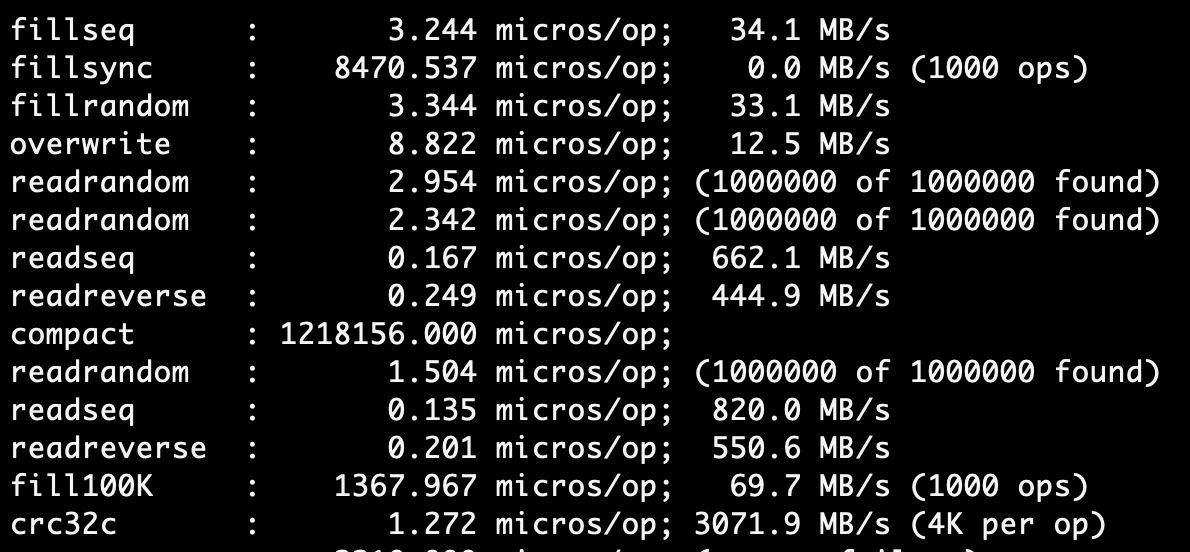
\includegraphics[width=0.31\textwidth]{./db_bench_blocksize_1KB.png}
        \label{fig:ae}
    }
    \subfloat[block size = 4 KB]{
        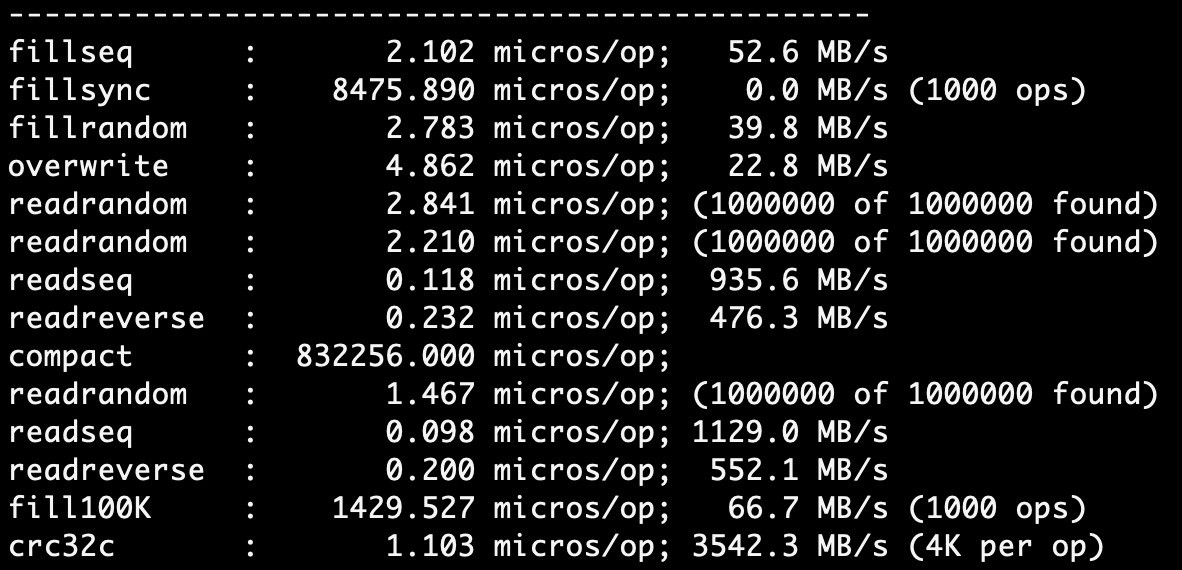
\includegraphics[width=0.3\textwidth]{./db_bench_blocksize_4KB.png}
        \label{fig:af}
    }
    \subfloat[block size = 16 KB]{
        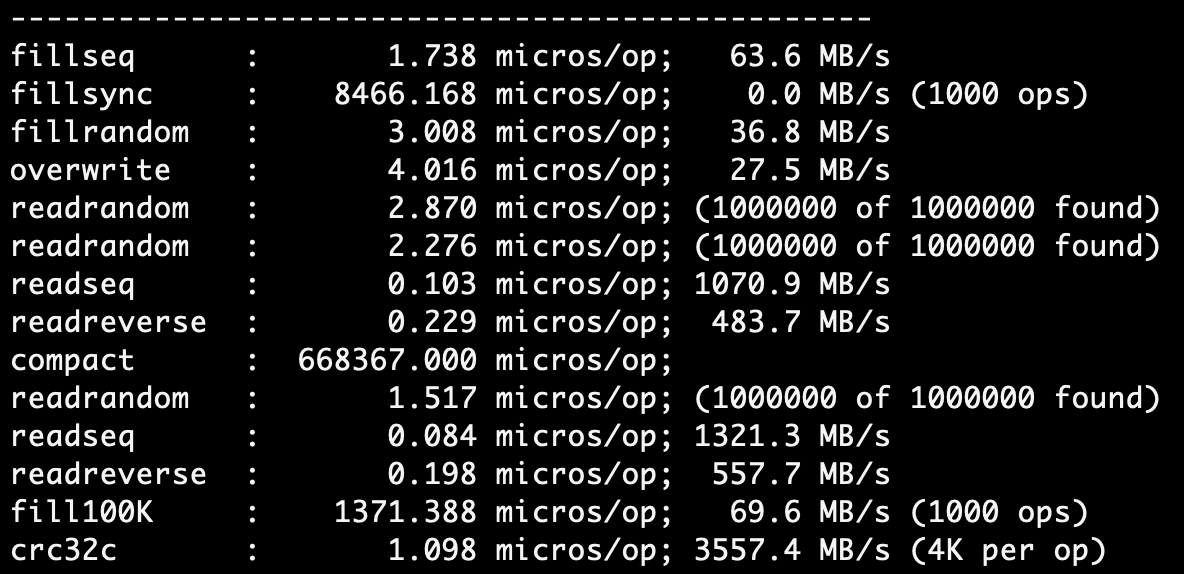
\includegraphics[width=0.3\textwidth]{./db_bench_blocksize_16KB.png}
        \label{fig:af}
    }
  \end{center}
  \caption{Experiment results of changing block\_size}
  \label{block_size}
\end{figure*}

\begin{figure*}[!htbp]
  \begin{center}
    \subfloat[write buffer size = 1 MB]{
        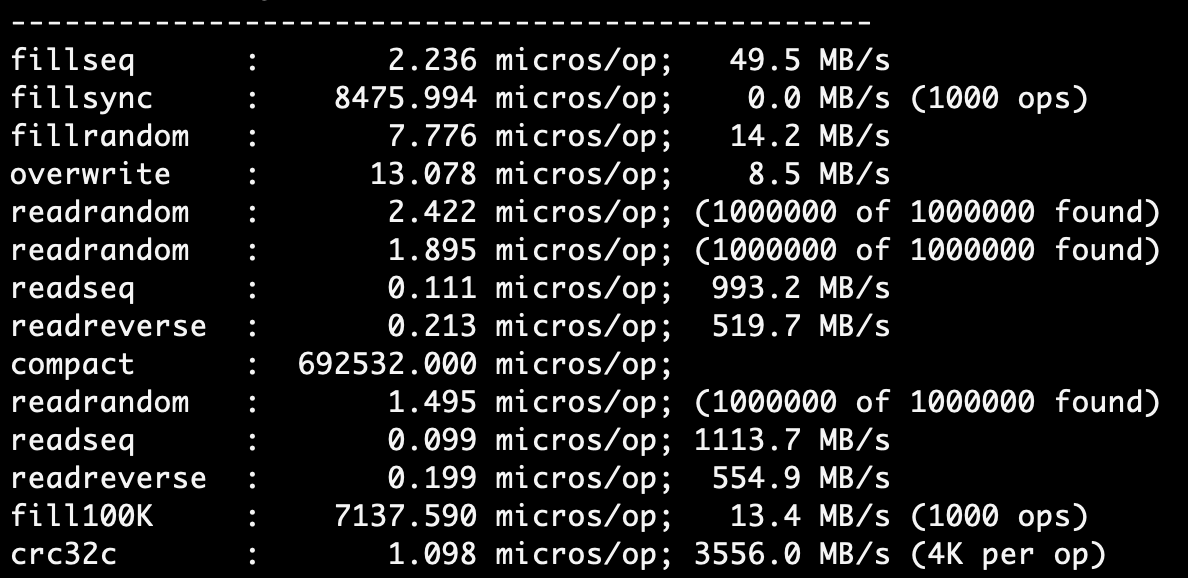
\includegraphics[width=0.3\textwidth]{./buffer_size_1MB.png}
        \label{fig:ae}
    }
    \subfloat[write buffer size = 4 MB]{
        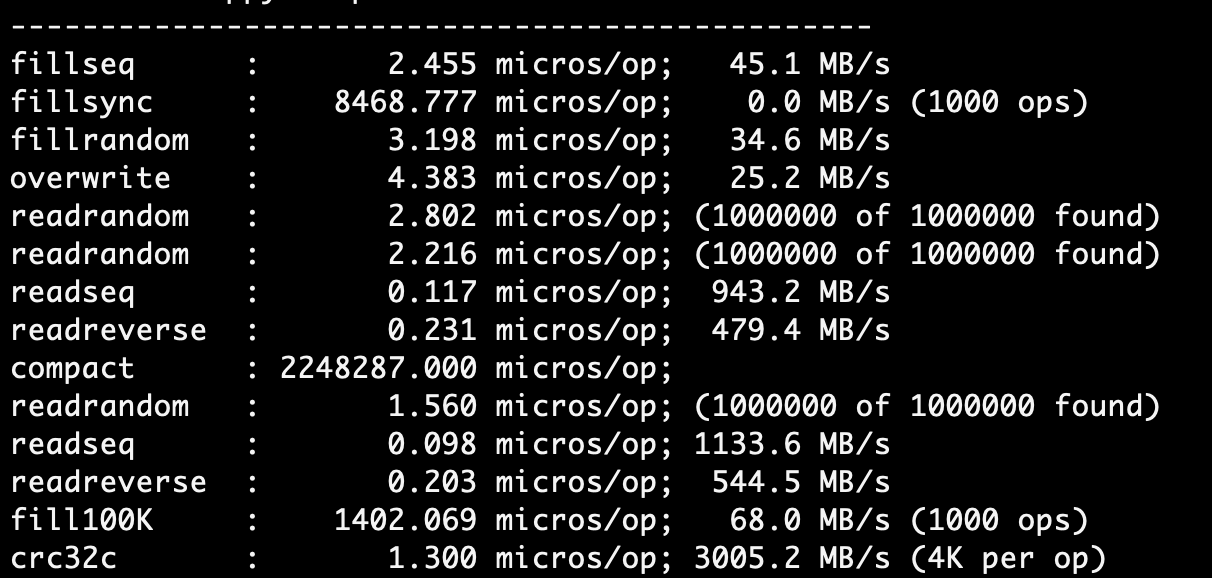
\includegraphics[width=0.3\textwidth]{./buffer_size_4MB.png}
        \label{fig:af}
    }
    \subfloat[write buffer size = 16 MB]{
        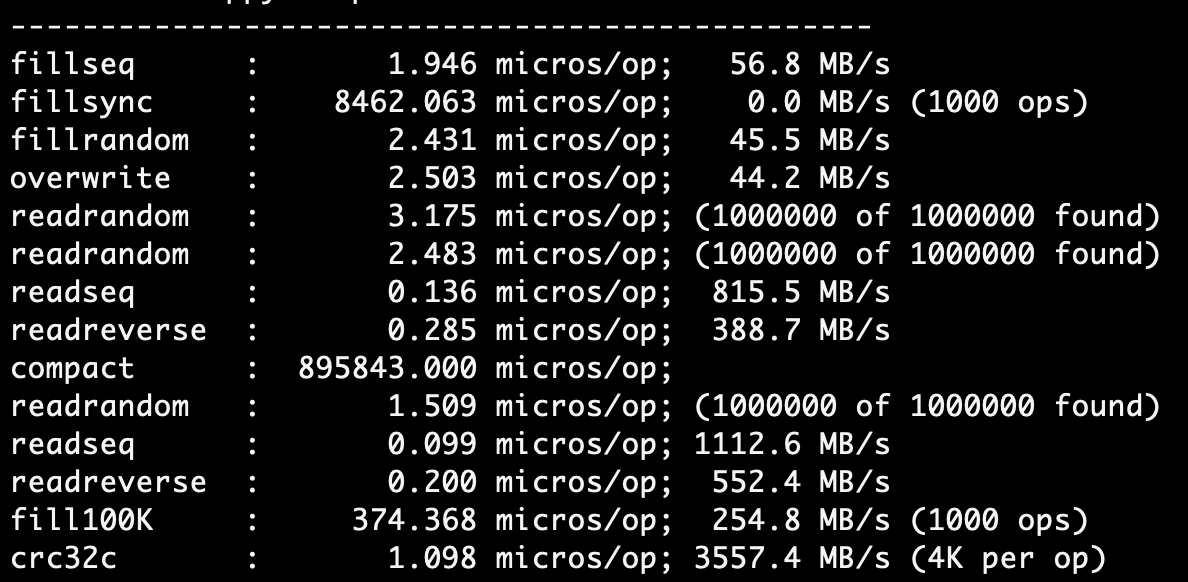
\includegraphics[width=0.3\textwidth]{./buffer_size_16MB.png}
        \label{fig:af}
    }
  \end{center}
  \caption{Experiment results of changing write\_buffer\_size}
  \label{buffer_size}
\end{figure*}

\begin{figure*}[!htbp]
  \begin{center}
    \subfloat[value size = 10 bytes]{
        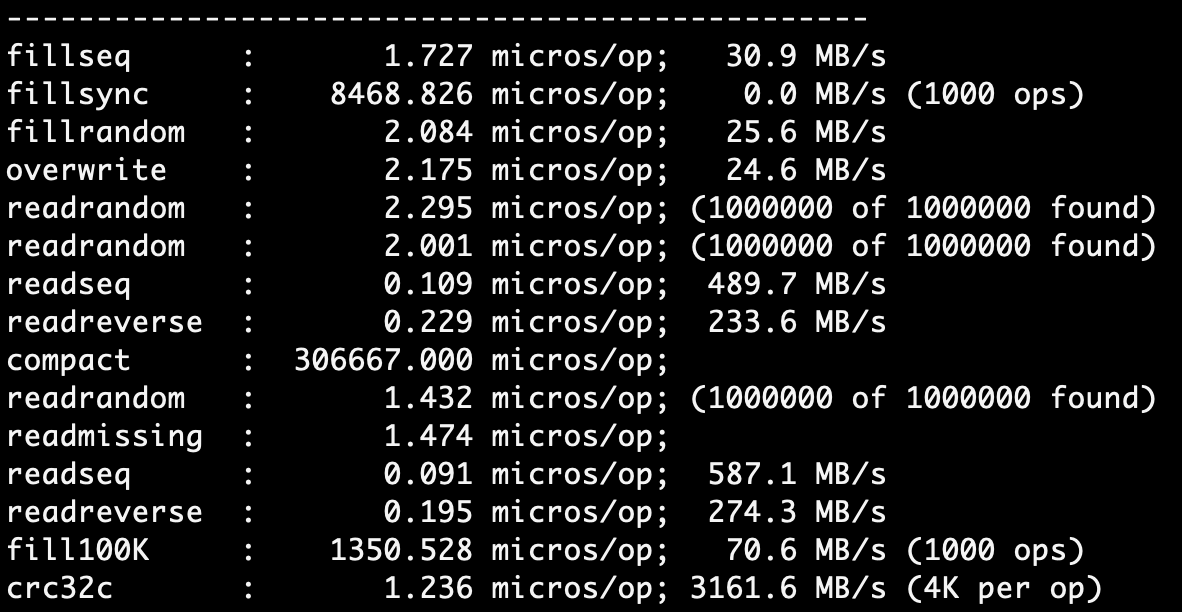
\includegraphics[width=0.3\textwidth]{./value_size_10B.png}
        \label{fig:ae}
    }
    \subfloat[value size = 20 bytes]{
        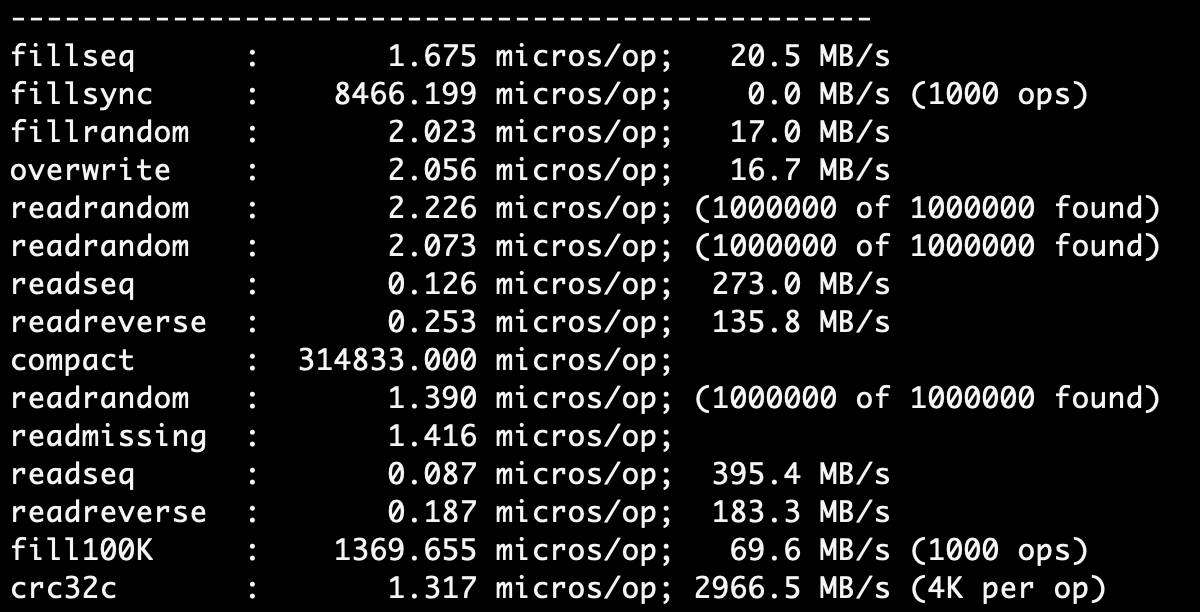
\includegraphics[width=0.3\textwidth]{./value_size_20B.png}
        \label{fig:af}
    }
    \subfloat[value size = 40 bytes]{
        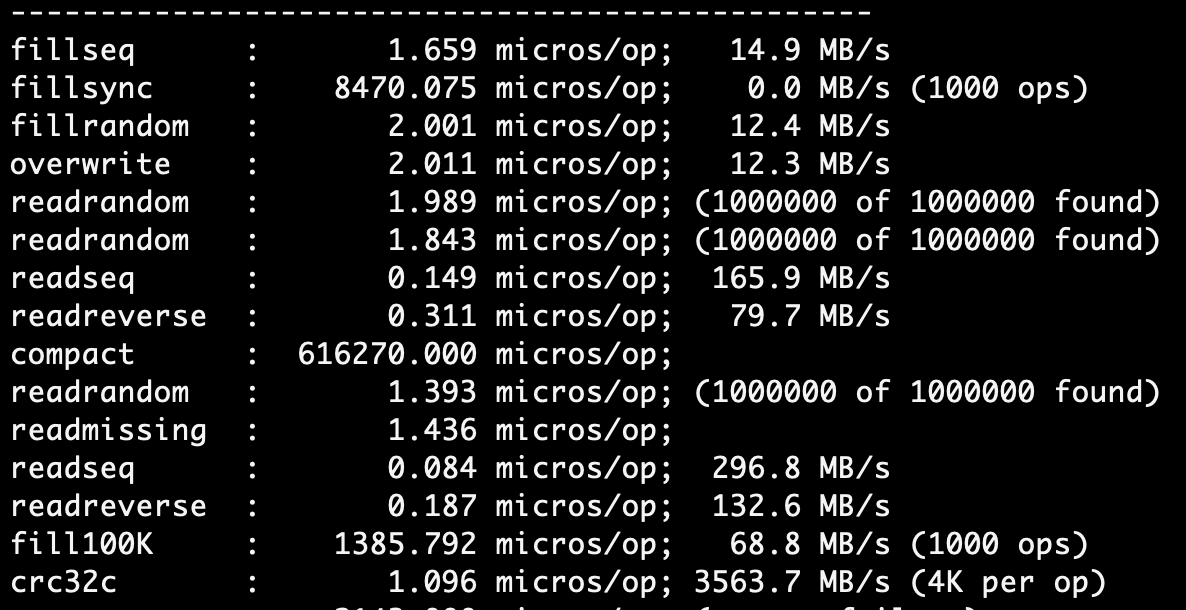
\includegraphics[width=0.3\textwidth]{./value_size_40B.png}
        \label{fig:af}
    }
  \end{center}
  \caption{Experiment results of changing value\_size}
  \label{value_size}
\end{figure*}

%-------------------------------------------------------------------------------
\section{Evaluation Results}
\label{sec:evaluation}
%-------------------------------------------------------------------------------
In this section, we evaluate the experiment results of each option.

In Figure~\ref{block_size}, the \textit{block\_size} is varied from 1 KB, 4 KB, to 16 KB. The performance metrics printed by \textit{db\_bench} shows that write-related metrics are affected by this options, for example, with the increased block size, overhead of sequential write in asynchrous mode (\textit{fillseq}) is reduced from 3.244 us to 2.102 us, and overhead of random write in in asynchrous mode (\textit{fillrandom}) is reduced from 3.334 us to 2.783 us. However, read-related metrics are not affected. Therefore, based on the result, we can tell that the larger block size it is, the smaller overhead of write operations in in asynchrous mode LevelDB wil have. 

In Figure~\ref{buffer_size}, the \textit{write\_buffer\_size} is varied from 1 MB, 4 MB, to 16 MB. It can be seen that write-related metrics are influenced, including \textit{fillseq}, \textit{fillrandom}, \textit{overwrite},etc. This observation can be explained by that large write buffer size can reduce the frequency of disk operations when encountered write opeations. However, increasing write buffer size has the side-effect of increasing the overhead of read-related operations, for instance, random read (\textit{readrandom}), sequential read (\textit{readseq}), reverse read (\textit{readreverse}) all are slightly increased when the write buffer size is enlarged.
 
In Figure~\ref{value_size}, the \textit{value\_size} is varied from 10 bytes, 20 bytes, to 40 bytes. It can be seen that the metric of compaction is affected by this option, with the growing of \textit{value\_size}, the overhead of compaction operation is increased as well, which grows from 306 ms to 616 ms eventually. This observation can be explained by that large value size makes compaction process take more effort to compress the object.  

\section{Conclusion}
\label{sec:conclusion}
In this report, we investigated the options provided by LevelDB. To understand how each option affects the system's performance, we selected 3 options, \textit{block\_size}, \textit{write\_buffer\_size} and \textit{value\_size} and conducted experiments by changing each option to different values to do the comparison, the results show that \textit{block\_size} affects write performance while not affect read performance, similarly, \textit{write\_buffer\_size} affects write performace, it also slightly affects read performance. Finally, \textit{value\_size} affects the compaction overhead.  

{\footnotesize 
\bibliographystyle{acm}
\bibliography{p1}
}
\end{document}
